\let\negmedspace\undefined
\let\negthickspace\undefined
\documentclass[journal]{IEEEtran}
\usepackage[a5paper, margin=10mm, onecolumn]{geometry}
%\usepackage{lmodern} % Ensure lmodern is loaded for pdflatex
\usepackage{tfrupee} % Include tfrupee package

\setlength{\headheight}{1cm} % Set the height of the header box
\setlength{\headsep}{0mm}     % Set the distance between the header box and the top of the text

\usepackage{gvv-book}
\usepackage{gvv}
\usepackage{cite}
\usepackage{amsmath,amssymb,amsfonts,amsthm}
\usepackage{algorithmic}
\usepackage{graphicx}
\usepackage{textcomp}
\usepackage{xcolor}
\usepackage{txfonts}
\usepackage{listings}
\usepackage{enumitem}
\usepackage{mathtools}
\usepackage{gensymb}
\usepackage{comment}
\usepackage[breaklinks=true]{hyperref}
\usepackage{tkz-euclide} 
\usepackage{listings}
% \usepackage{gvv}                                        
\def\inputGnumericTable{}                                 
\usepackage[latin1]{inputenc}                                
\usepackage{color}                                            
\usepackage{array}                                            
\usepackage{longtable}                                       
\usepackage{calc}                                             
\usepackage{multirow}                                         
\usepackage{hhline}                                           
\usepackage{ifthen}                                           
\usepackage{lscape}
\begin{document}

\bibliographystyle{IEEEtran}
\vspace{3cm}

\title{4.7.14}
\author{EE25btech11028 - J.Navya sri}
% \maketitle
% \newpage
% \bigskip
{\let\newpage\relax\maketitle}


\textbf{Question:} \\
Find the distance of the plane 
2x - 3y + 4z - 6 = 0
from the origin.


\bigskip


\textbf{Solution:} \\
We want to find the distance of the plane 
\begin{equation}
2x - 3y + 4z - 6 = 0 \quad \text{(1)}
\end{equation} 
from the origin using the vector approach

\vspace{0.5em}
\textbf{Step 1: Identify the normal vector.}

The general equation of a plane is 
\begin{equation}
\mathbf{n} \cdot \mathbf{r} = D \quad \text{(2)}
\end{equation}
where 
\begin{equation}
\mathbf{n} = \begin{pmatrix} A \\ B \\ C \end{pmatrix} \quad \text{(3)}
\end{equation} 
is the normal vector of the plane and $D$ is a constant. 

From the given plane ($2x - 3y + 4z = 6$), we have
\begin{equation}
\mathbf{n} = \begin{pmatrix} 2 \\ -3 \\ 4 \end{pmatrix}, \quad D = 6. \quad \text{(4)}
\end{equation}

\vspace{0.5em}
\textbf{Step 2: Distance formula.}

The distance of a point $\mathbf{r}_0$ from the plane is given by
\begin{equation}
\text{Distance} = \frac{|\mathbf{n} \cdot \mathbf{r}_0 - D|}{\|\mathbf{n}\|} \quad \text{(5)}.
\end{equation}

For the origin, $\mathbf{r}_0 = \begin{pmatrix} 0 \\ 0 \\ 0 \end{pmatrix}$, so
\begin{equation}
\begin{split}
\text{Distance} &= \frac{|\mathbf{n} \cdot \mathbf{r}_0 - 6|}{\sqrt{2^2 + (-3)^2 + 4^2}} \\
&= \frac{|(2)(0) + (-3)(0) + (4)(0) - 6|}{\sqrt{4 + 9 + 16}} \\
&= \frac{|-6|}{\sqrt{29}} = \frac{6}{\sqrt{29}} \quad \text{(6)}.
\end{split}
\end{equation}

\vspace{0.5em}
\textbf{Answer:}
\begin{equation}
\boxed{\frac{6}{\sqrt{29}}} \quad \text{(7)}
\end{equation}

\textbf{Graph presentation:}
\begin{figure}[H]
\begin{center}
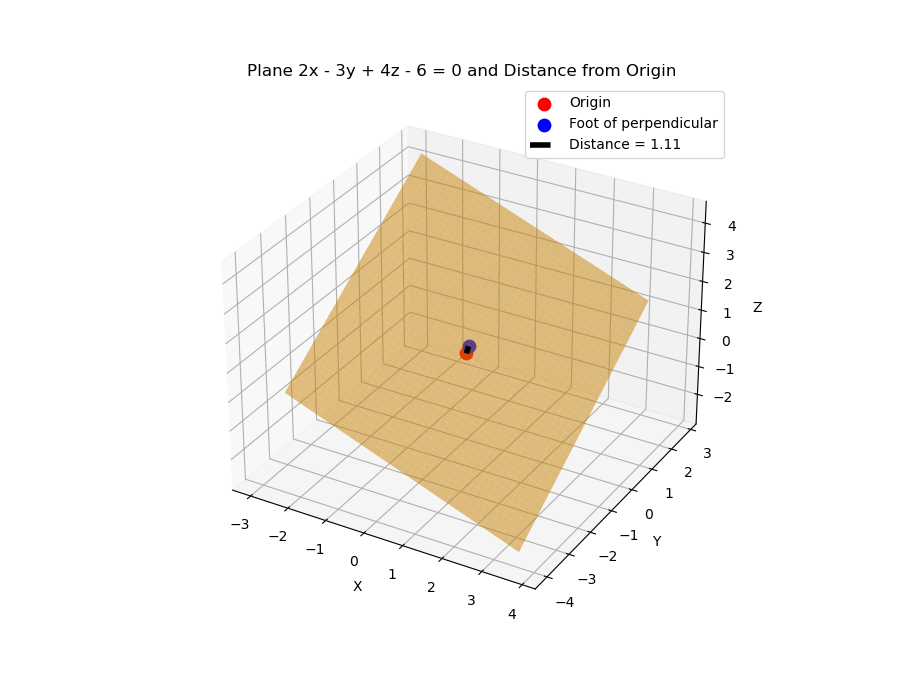
\includegraphics[width=0.6\columnwidth]{Figs/fig7.png}
\end{center}
\caption{}
\label{fig:Fig}
\end{figure}
\end{document}